\documentclass{article}
\usepackage{fasy-hw}
\usepackage{hyperref}
\usepackage{graphicx}

\author{Joshua Harthan}
\problem{1}
\collab{none}
\begin{document}
8.1 Question 20 
\item[] Let $A$ = \{-1,1,2,4\} and $B$ = \{1,2\} and define relations $R$ and $S$ and from $A$ to $B$ as follows: For all $(x,y)\; \epsilon \; A \; \times \; B$,

$$\item[] x\;R\;y \; \;\Leftrightarrow \; \; |x|=|y| \;  and $$
$$x \; S \; y \; \;\Leftrightarrow \; \; x-y \; is \; even $$
\item[]State explicitly which ordered pairs are in $A$ \times \;$B$, \; $R$, \; $S$, \; $R \cup \; S$, and $R\cap S$.
\item[]From the relations given, we can see that R\{(-1,1), (1,1),(2,2)\}, since these sets satisfy the quality $|x|=|y|$,  and S\{(-1,1),(4,2)\}, since these sets qualify $x-y$ is even. $A \times B$ is the set of numbers \{(-1,1),(-1,2),(1,1),(1,2),(2,1),(2,2),(4,1),(4,2)\}. $R \; \cap \; S$ is the set of numbers \{(-1,1)\}, as the intersection of sets $R$ and $S$ are the numbers in common between the sets. $R \; \cap \; S$ is the set of numbers \{(-1,1),(1,1),(2,2),(4,2)\} as the intersection of sets $R$ and $S$ are all the sets of numbers that are in both sets. 

\problem{2}
\collab{none}
\clearpage
\header
8.2 Question 21
\item[]Determine whether the given relation is reflexive, symmetric, transitive, or none of these. Justify your answer.
\item[]Let $X$ = $\{a,b,c\}$ and $P(X)$ be the power set of $X$. A relation \textbf{L} is defined on $P(X)$ as follows: For all {\tiny {A,B}} $\epsilon$ \;  $P(X)$, {\tiny A} \textbf{L} {\tiny B} $\Leftrightarrow$ the number of elements in {\tiny A} is less than the number of elements in {\tiny B}.
\item[]The power set $P(X)$ is defined to be the set \{(), (a), (b), (c), (a,b), (a,c), (b,c), (a,b,c)\}. In this case, the relation would be neither reflexive, symmetric, nor transitive. This is due to the fact set $A$ has less elements than that in set $B$, meaning that the number of elements in each set cannot be equal. Because the number of elements is not equal, this implies that none of the relations cannot be reflexive, symmetric, or transitive, as these all imply equality.


\problem{3}
\collab{none}
\clearpage
\header
8.3 Question 23
\item[]Find the distinct equivalence classes of $R$.
\item[] $R$ is the relation defined on \textbf{Z} as follows: For all ($m$, $n$) $\epsilon$ \textbf{Z},
$$
m \; R \; n \; \Leftrightarrow \; 4|(m^{2} - n^{2}). 
$$
\item[] Reflexive:
\item[] To show that $R$ is reflexive, we must show that for all $m$ $\epsilon$ $\textbf{Z}$, $m^{2} \; R \; m^{2}$. By the definition of $R$, this means that for all $m$ $\epsilon$ $\textbf{Z}$, $4|(m^{2} - m^{2}) = 4|0.$ This is true for $4|0$ since $4 \times 0  = 0$. Therefore $R$ is reflexive.
\item[] Symmetric:
\item[] To show that $R$ is symmetric, we must show that for all $m, n$ $\epsilon$ $\textbf{Z}$ if $m^{2} \; R \; n^{2}$ then $n^{2} \; R \; m^{2}$. By the definition of $R$ this means that for  $m, n$ $\epsilon$ $\textbf{Z}$ if $4|(m^{2} - n^{2})$ then $4|(n^{2} - m^{2})$. This is true, since $m^{2} - n^{2}$ = ($m - n$)($m + n$) for all integers $m$ and $n$, therefore 4$|(m - n)$ or 4$|(m + n)$. From this we see that either $m - n = 4x$ or $m + n = 4x$ for some integer $x$.From these equations, it can be seen that -$(m^{2} - n^{2})$ = -4$x$ which equals $(n^{2} - m^{2})$ = 4$(-x)$. Since -$x$ is an integer, we can say that 4$|(n^{2} - m^{2})$. Therefore, $R$ is symmetric.
\item[] Transitive:
\item[] To show that $R$ is transitive, we must show that for all $m, n, p$ $\epsilon$ $\textbf{Z}$ if $m^{2} \; R \; n^{2}$ and $n^{2} \; R \; p^{2}$ then $m^{2} \; R \; p^{2}$. By definition of $R$ this means that for all $m, n, p$ $\epsilon$ $\textbf{Z}$, if 4$|(m^{2} - n^{2})$ and 4$|(n^{2} - p^{2})$, then 4$|(m^{2} - p^{2})$. This is true since 4$|(m^{2} - n^{2})$ and 4$|(n^{2} - p^{2})$ implies $m^{2} - n^{2} = 4y$ and $n^{2} - p^{2} = 4z$ for some integers $y$ and $z$. Adding these two equations together leads to $(m^{2} - n^{2}) + (n^{2} - p^{2}) = 4y + 4z$, which is equivalent to $m^{2} - p^{2} = 4(y+z)$. Since $y$ and $z$ are integers, so is $y + z$. This shows that 4$|(m^{2} - p^{2})$. Therefore, $R$ is transitive. 


\problem{4}
\collab{none}
\clearpage
\header
2.1 Question 20
\item[]Determine whether the statement forms in 16-24 are logically equivalent. In each case, construct a truth table and include a sentence justifying your answer.
$$p \; \land \; c \;\; and \;\; p \; \lor \; c $$ 
\begin{figure}[h!]
  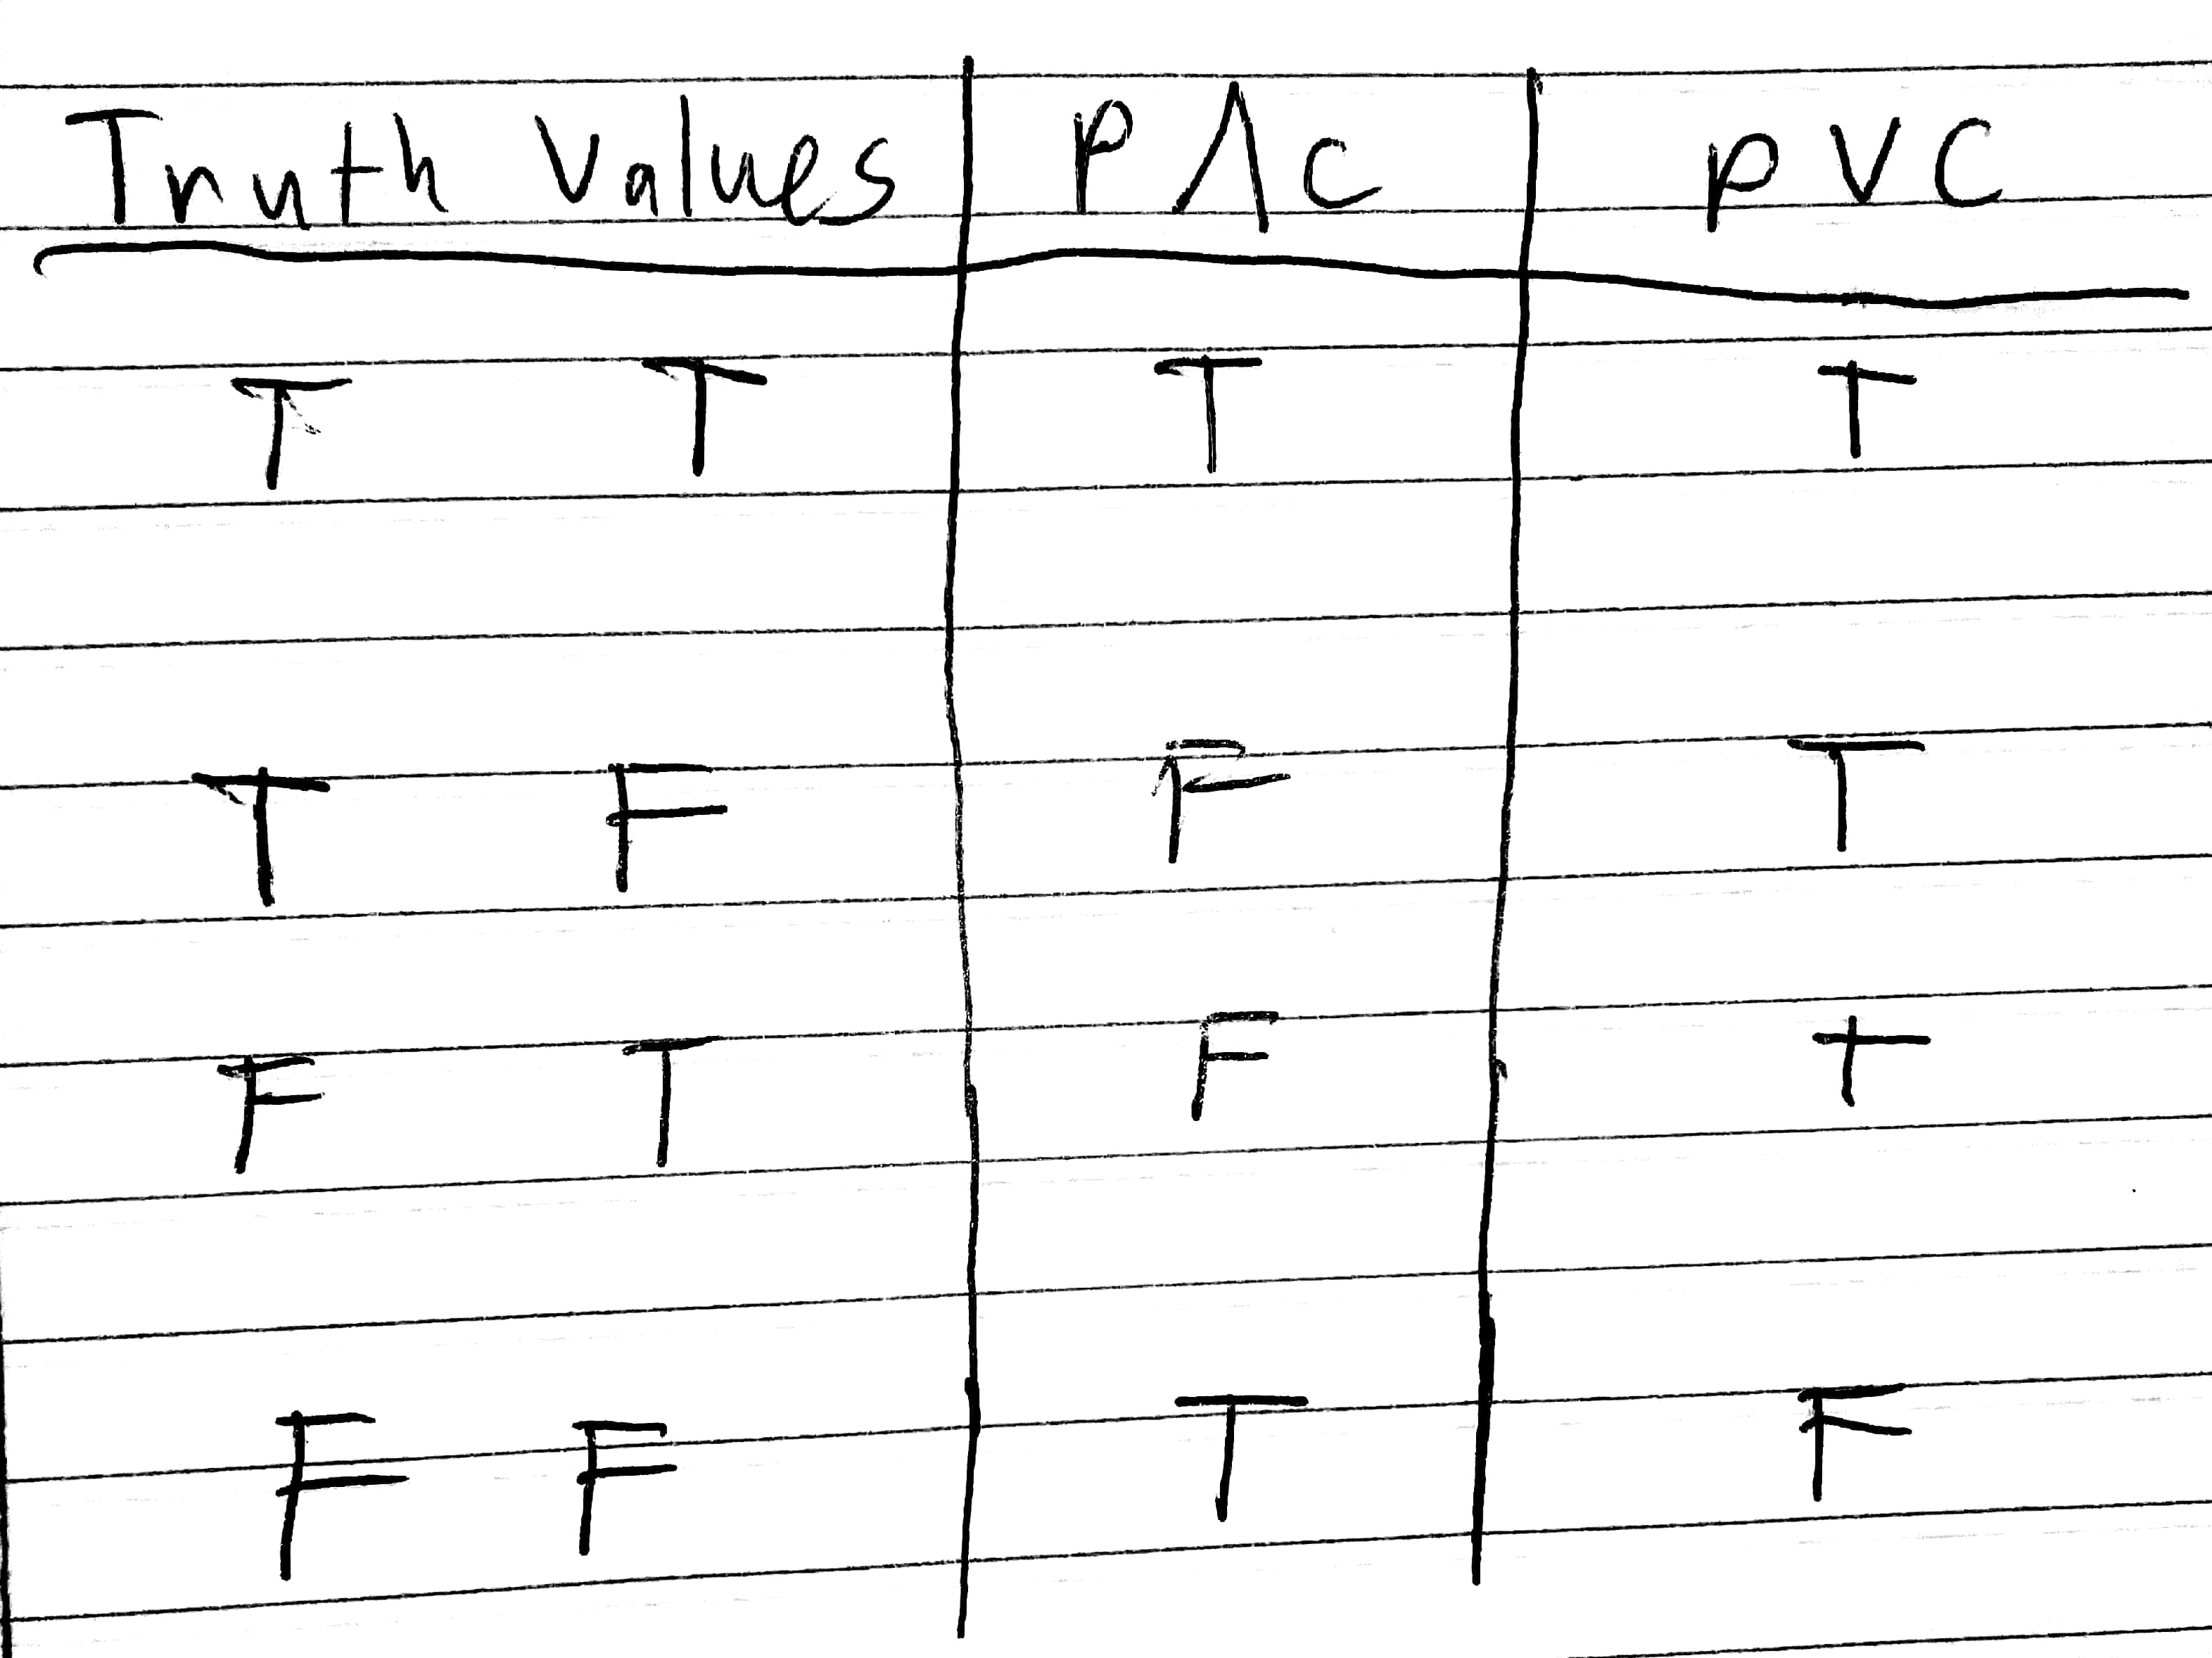
\includegraphics[width=\linewidth]{tt1.jpg}
  \caption{Truth Table showing $p \; \land \; c \;\; and \;\; p \; \lor \; c $}
  \label{fig:table1}
\end{figure}
\item[] From this table, it can be seen that $p \; \land \; c \;\; and \;\; p \; \lor \; c $ are not equivalent statements, as they have different outputs for the same truth values that were input.


\problem{4 cont.}
\collab{none}
\clearpage
\header
2.1 Question 22
\item[]Determine whether the statement forms in 16-24 are logically equivalent. In each case, construct a truth table and include a sentence justifying your answer.
$$p \; \land \; (q \; \lor \; r) \;\; and \;\; (p\;\land \; q) \; \lor \; (p \; \land \; r)$$ 
\begin{figure}[h!]
  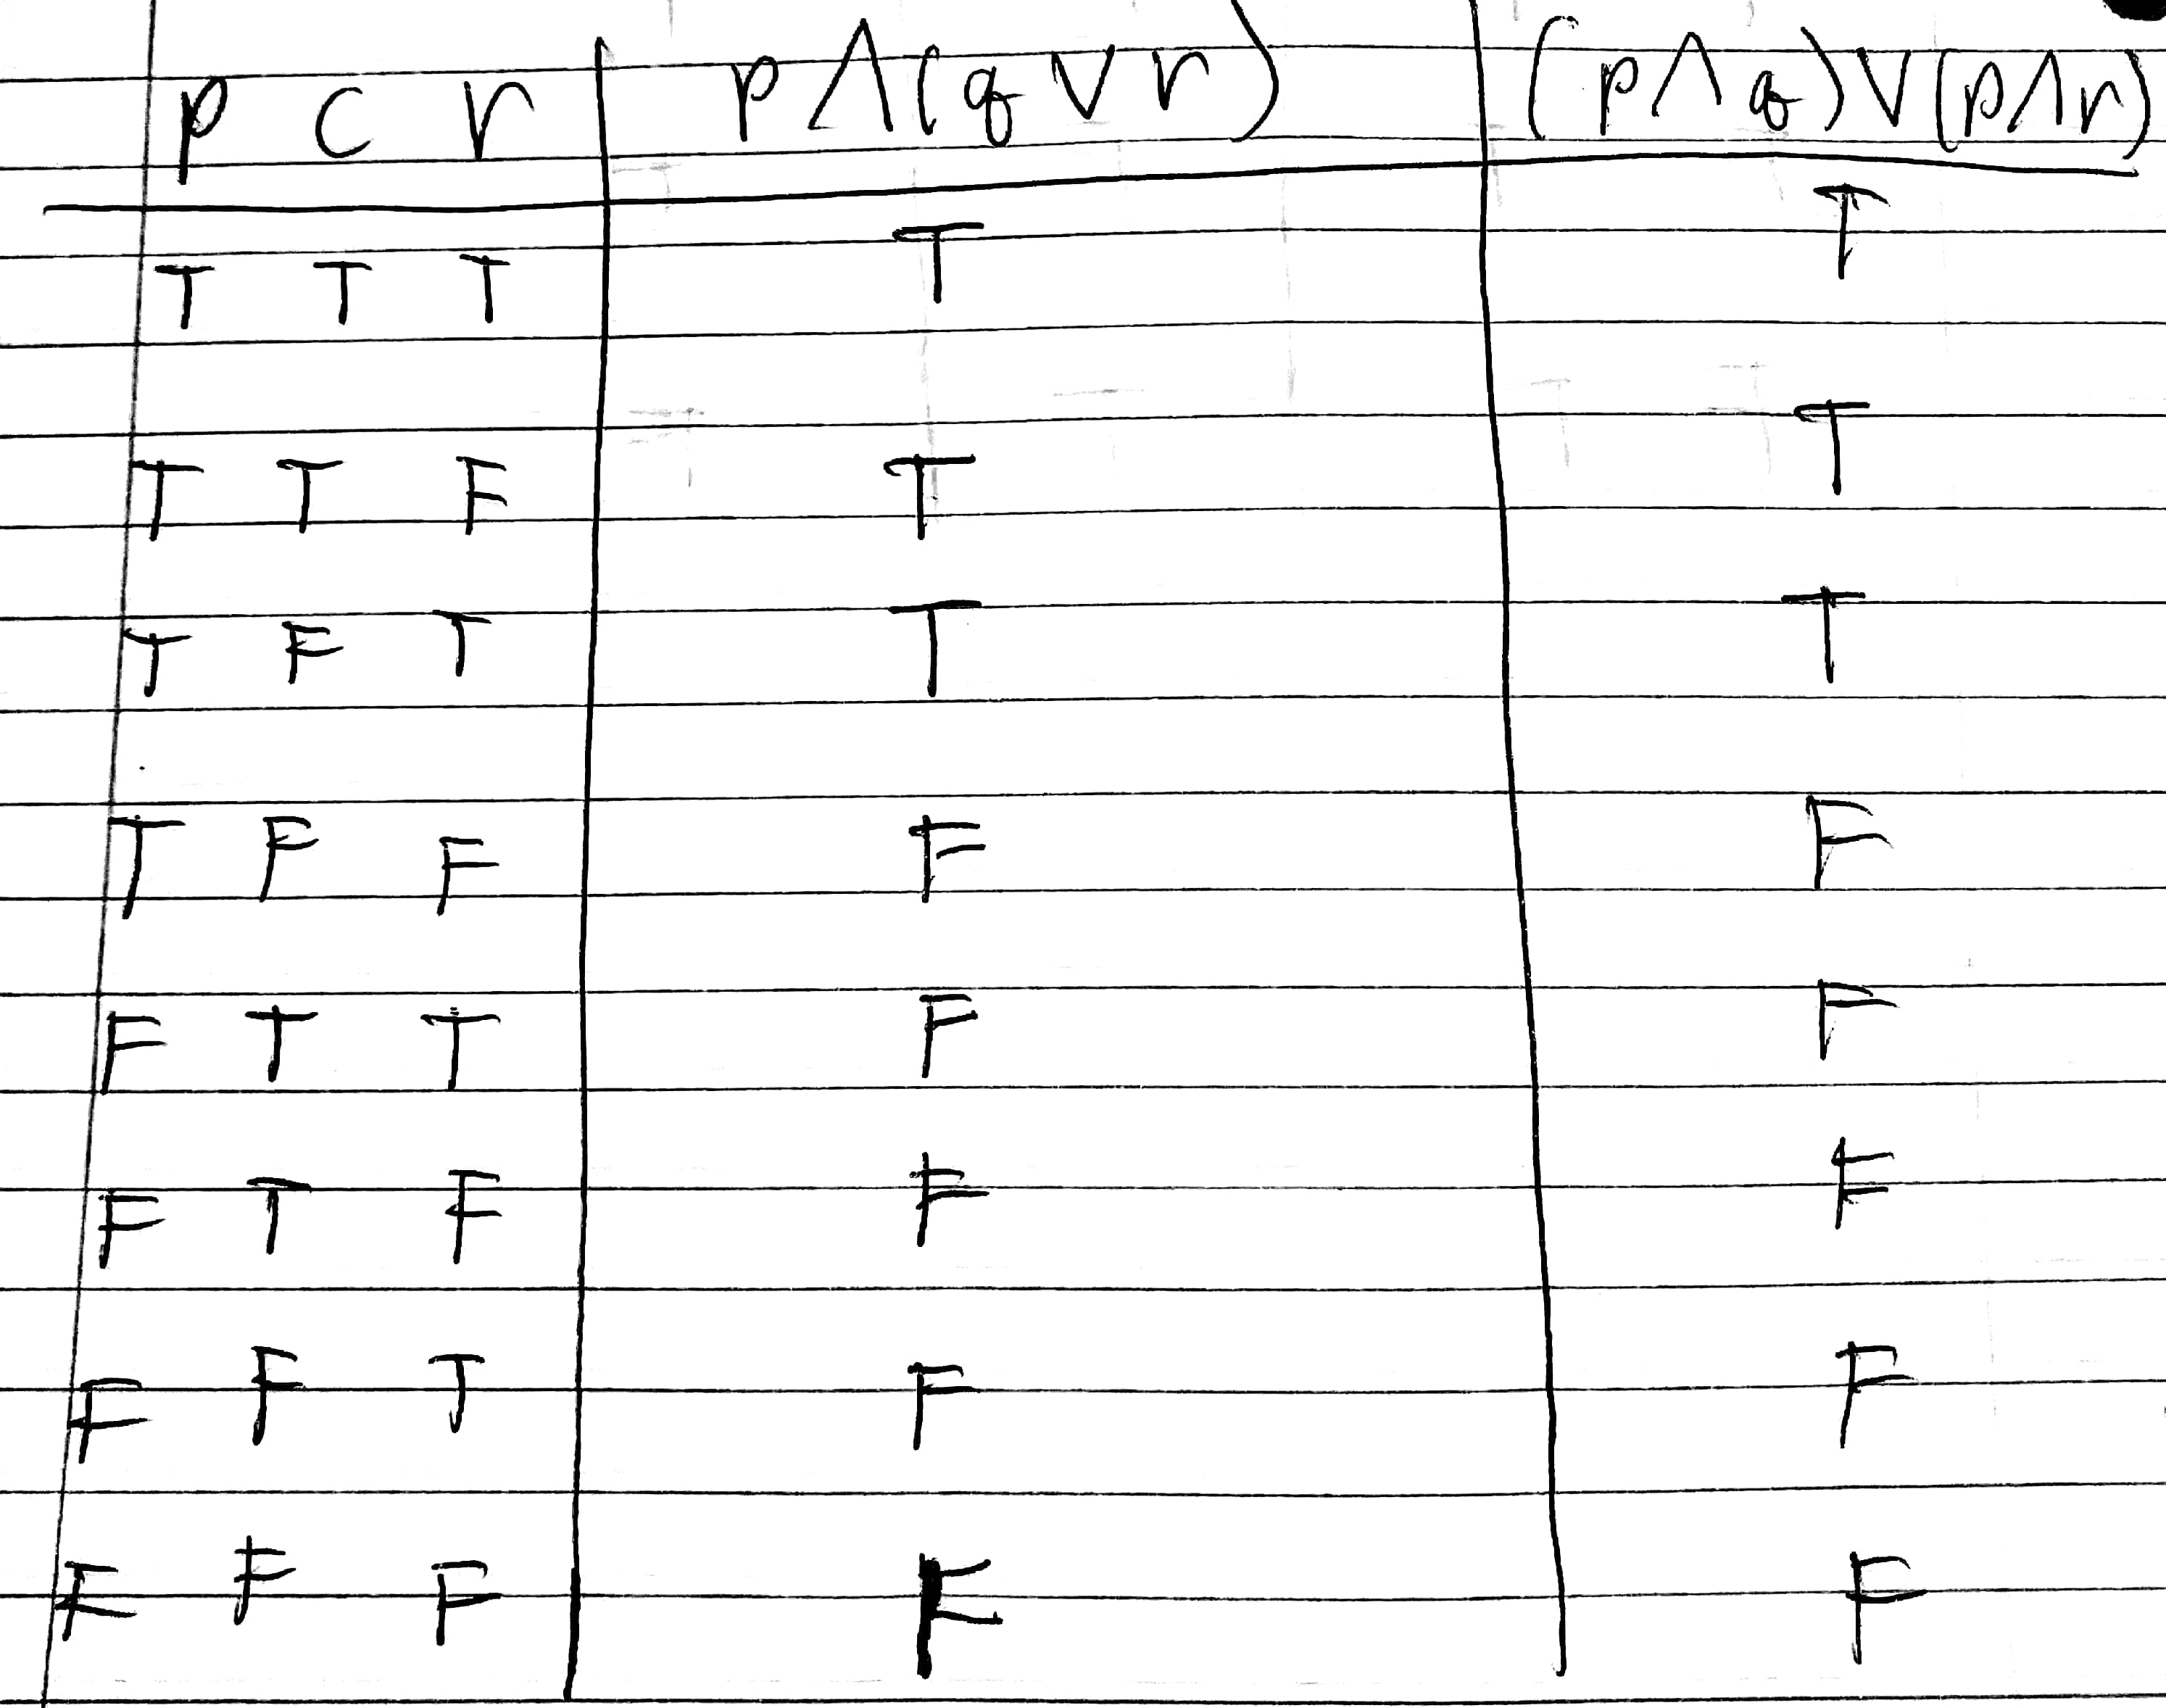
\includegraphics[width=\linewidth]{tt2.jpg}
  \caption{Truth Table showing $p \; \land \; (q \; \lor \; r)$ and $(p\;\land \; q) \; \lor \; (p \; \land \; r)$}
  \label{fig:table2}
\end{figure}
\item[] From this table, it can be seen that $p \; \land \; (q \; \lor \; r) $ and  $(p\;\land \; q) \; \lor \; (p \; \land \; r)$ are logically equivalent, as they have the same outputs for the same truth values that were input.


\problem{5}
\collab{none}
\clearpage
\header
2.3 Question 40
\item[]Sharky, a leader of the underworld, was killed by one of his own band of four henchmen. Detective Sharp interviewed the men and determined that all were lying except for one. He deduced who killed Sharky on the basis of the following statements: 
\item[] a. Socko: Lefty killed Sharky.
\item[] b. Fats: Muscles didn't kill Sharky.
\item[] c. Lefty: Muscles was shooting craps with Socko when Sharky was knocked off.
\item[] d. Muscles: Lefty didn't kill Sharky.
\item[] Who did kill Sharky?
\item[]From these statements, we can find that Muscles killed Sharky. We know this because, from viewing the statements that each individual gave, statements a. and d. conflict with each other. Because we also know that every person but one is lying, we know that either a. or d. is the truth, since they are conflicting statements. Since we know that either of these statements are true, we know that the statments b. and c. are definitely false. Since we know both of these statements are false, and statement b. states that Muscles didn't kill Sharky, we know that Muscles did in fact kill Sharky. Statement c. states that Muscles was shooting craps with Socko when Sharky was killed, so we know that Muscles was in fact not shooting craps when Sharky was killed. Therefore, from these statements, we know that Muscles killed Sharky. 

\problem{6}
\collab{none}
\clearpage
\header
4.5 Question 29
\item[] Prove the statement by (a) contraposition and (b) contradiction:
\item[]For all integers $a$, $b$, and $c$ if $a$ $\mid$ $b$ and $a$ $\nmid$ $c$, then $a \nmid (b + c)$.
\item[](a) To argue by contrapostion, we must take the contrapositive of these statements, therefore we suppose $a \nmid b$ and $a$ $\mid$ $c$ is true. We can disprove this by supposing that $a$ = 10, $b$ = 8, $c$ = 2. 10$\mid$ 8 leads to a non-integer, while 10$\mid$2 leads to an integer 5. This stays in line with  $a$ $\nmid$ $b$ and $a$ $\mid$ $c$ we supposed. However, 10 $\mid$ (8+2) or 10 $\mid$ 10 leads to an integer, which disproves the statement $a \nmid (b + c)$. Therefore, since $a \nmid (b + c)$ is false for the statements $a \nmid b$ and $a$ $\mid$ $c$, $a \nmid (b + c)$ must be true for the statements $a$ $\mid$ $b$ and $a$ $\nmid$ $c$.
\item[](b) To contradict this statement we must suppose that the statement $a \nmid (b + c)$ is false, i.e. suppose that $a \mid (b + c)$ is true. We can contradict this statement by supposing that $a$ = 4, $b$ = 2, $c$ = 3. 4$\mid$ 2 leads to an integer 2, while 4$\mid$3 does not lead to an integer. This stays in line with  $a$ $\mid$ $b$ and $a$ $\nmid$ $c$ given. However, 4 $\mid$ (2+3) or 4 $\mid$ 5 leads to a non-integer, which contradicts the statement $a \mid (b + c)$. Therefore, since $a \mid (b + c)$ is false, $a \nmid (b + c)$ must be true.

\problem{7}
\collab{none}
\clearpage
\header
\item[] References to online resources are provided as footnotes
\item[]Augustus De Morgan is a British mathematician and logician, most known for his contributions to computer science through his formulation of De Morgan's Laws, a set of laws that deal with boolean algebra. Since boolean algebra is the basis of logic gates, which are the basis of logic circuits and therefore computation, De Morgan's Laws has helped in the field of computer science by allowing in the manipulation of sets through negation. Without De Morgan's Laws, we would not have easier simplifications of computer program logic, as well as not have easier simplification in logic circuit design.
\item[]
\item[]
\item[] 
\item[]
\item[] 
\item[] 
\item[]
\item[] 
\item[] 
\item[]
\item[] 
\item[] 
\item[]Online Resources:
\item[]\url{https://en.wikipedia.org/wiki/Augustus_De_Morgan}
\item[]\url{https://en.wikipedia.org/wiki/De_Morgan's_laws}

\end{document}